Um den Zugriff auf die Datenbank zu beschränken, wird zwischen die Datenschnittstelle und die Datenbank eine Benutzerverwaltung geschaltet. Diese überprüft nun bei jeder Anforderung auf einen Zugriff auf die Datenbank, ob dieser vom aktuellen Nutzer erlaubt ist oder nicht.
\begin{wrapfigure}{l}{0.4\textwidth}
	\vspace{-20pt}
\begin{center}
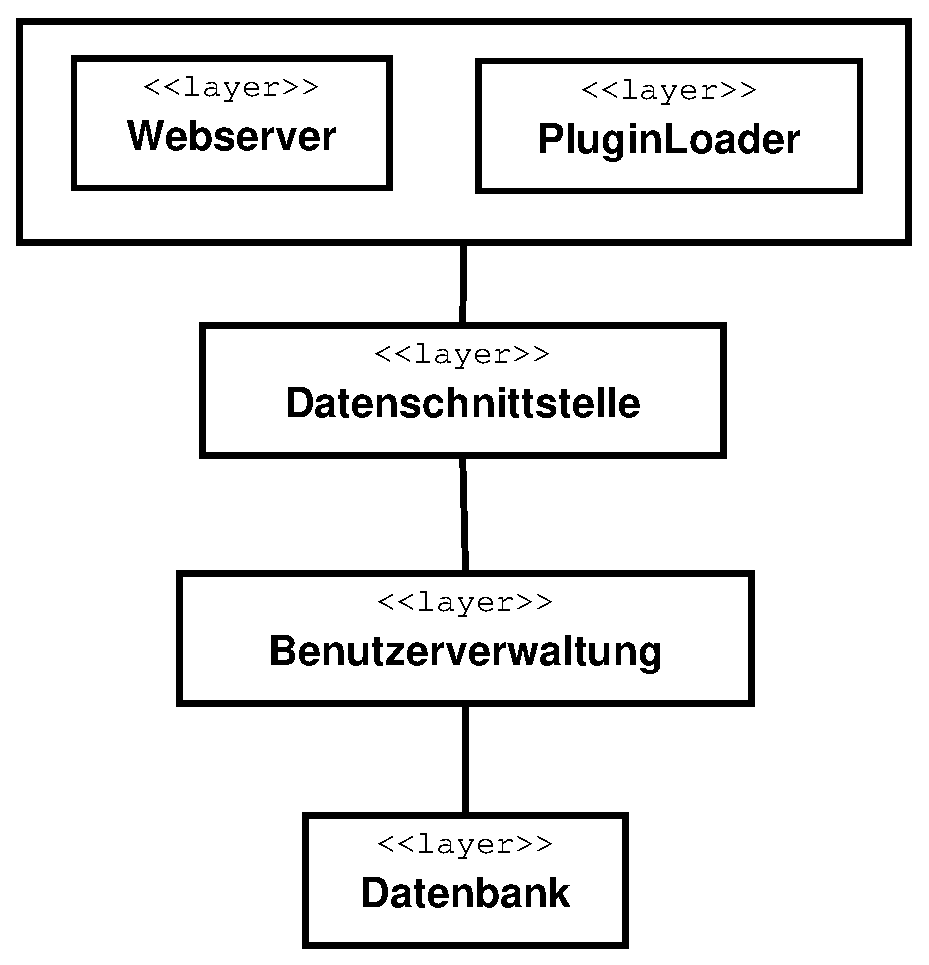
\includegraphics[width=1\linewidth]{Grafik/Diagramm/Layer}
\end{center}
\vspace{-15pt}
\caption[Layer-Klassen]{Layer-Pattern mit Benutzerverwaltung}
\label{fig:Layer}
\vspace{-50pt}
\end{wrapfigure}
\subsubsection{Was spricht für das Layer-Pattern}
Das Layer-Pattern hilft einen unerlaubten Zugriff auf die Datenbank zu verhindern und stellt sicher, dass jeder zugriff erst über die Benutzerschnittstelle erlaubt wird. Ein weiterer Vorteil stellt die Flexibilität der einzelnen Schichten dar, so kann die Datenschnittstelle statt der lokalen Datenbank auch die Datenbank eines anderen Servers über REST abrufen, da die Kommunikationswege innerhalb des Layer-Pattern identisch sind.
\vspace{30pt}